% Behaviour of the stator voltage and the RMS-value of the stator
% flux as a function of speed in scalar control.
% Author: Erno Pentzin (2013)
%\documentclass{article}
\documentclass[tikz,border=5pt]{standalone}
\usepackage{amsmath} % Required for \varPsi below
\usepackage{tikz}
\begin{document}

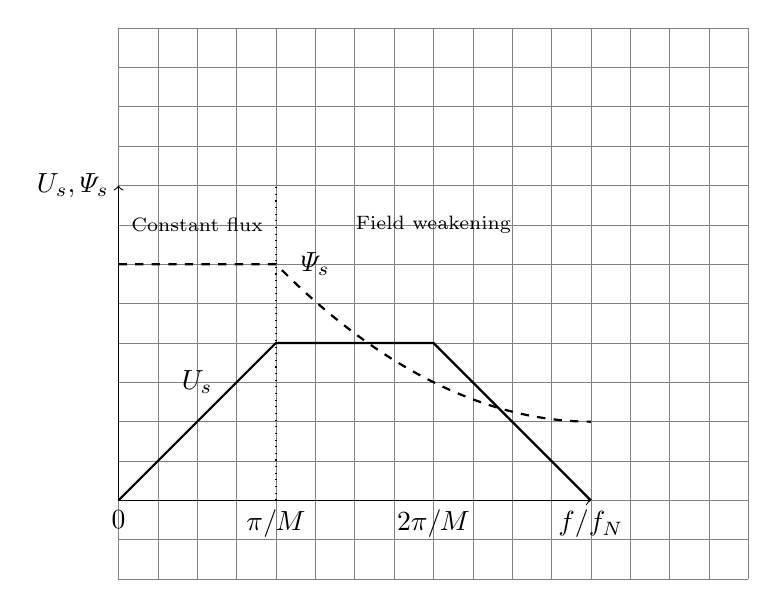
\begin{tikzpicture}
	\draw[step=0.5,help lines] (0,-1) grid (8,6);

% horizontal axis
\draw[->] (0,0) -- (6,0) node[anchor=north] {$f/f_N$};
% labels
\draw	(0,0) node[anchor=north] {0}
		(2,0) node[anchor=north] {$\pi/M$}
		(4,0) node[anchor=north] {$2\pi/M$};
% ranges
\draw	(1,3.5) node{{\scriptsize Constant flux}}
		(4,3.5) node{{\scriptsize Field weakening}};

% vertical axis
\draw[->] (0,0) -- (0,4) node[anchor=east] {$U_s,\varPsi_s$};
% nominal speed
\draw[dotted] (2,0) -- (2,4);

% Us
				\draw[thick] (0,0) -- (2,2) -- (4,2) -- (6,0);
\draw (1,1.5) node {$U_s$}; %label

% Psis
\draw[thick,dashed] (0,3) -- (2,3) parabola[bend at end] (6,1);
\draw (2.5,3) node {$\varPsi_s$}; %label

\end{tikzpicture}

\end{document}

